\chapter{工程基础}
\dirtree{%
.1 2 《Hands-On Machine Learning with Scikit-Learn, Keras \& TensorFlow》.
.2 = 把机器学习从"会解释"推进到"能做项目".
.3 0 工程工具层（把算法接到真实数据上）.
.4 数据清洗.
.4 Pipeline.
.4 训练/验证/测试切分.
.3 能力一 做一个完整机器学习项目 → 端到端流程.
.4 明确业务目标.
.4 构造特征.
.4 建立基线.
.3 能力二 训练传统模型 → sklearn 实战.
.4 线性模型 / SVM.
.4 决策树 / 随机森林.
.4 集成学习 / Boosting.
.3 能力三 训练神经网络 → 深度学习入门.
.4 MLP.
.4 CNN.
.4 RNN / Attention.
.3 能力四 调优与上线意识 → 让模型能用.
.4 Grid Search / Random Search.
.4 学习曲线与误差分析.
.4 保存模型、复现实验、监控效果.
}
\chapter{训练前的准备}














\chapter{训练前的设计}


\chapter{训练传统模型}

\section{回归树}
\begin{definition}[回归树]
回归树是一种非参数化的监督学习方法，用于预测连续型输出变量。它通过递归地划分输入特征空间，并在每个划分区域内用常数值（通常是该区域训练样本的均值）作为预测，从而构建一个分段常数函数近似目标函数。
\end{definition}
建立回归树的过程大致可以分为两步：

\begin{enumerate}
  \item 将预测变量空间（即 $X_1, X_2, \dots, X_p$ 的可能取值构成的集合）分割成 $J$ 个互不重叠的区域 $R_1, R_2, \dots, R_J$。
  \item 对落入区域 $R_j$ 的每个观测值做同样的预测，预测值等于 $R_j$ 上训练集的响应值的简单算术平均。
\end{enumerate}

举个例子，若在第一步中得到两个区域 $R_1$ 和 $R_2$，$R_1$ 上训练集的平均响应值为 $10$，$R_2$ 上训练集的平均响应值为 $20$。那么，对于给定的观测值 $X = x$，若 $x \in R_1$，则预测值为 $10$；若 $x \in R_2$，则预测值为 $20$。

现在详细说明上面的第一步。如何构建区域 $R_1, R_2, \dots, R_J$？理论上，区域的形状是任意的，但出于模型简化和增强可解释性的考虑，这里将预测变量空间划分成高维矩形，或称盒子（box）。划分区域的目标是找到使模型的残差平方和（RSS）最小的矩形区域 $R_1, R_2, \dots, R_J$。

RSS 的定义为
\[
\sum_{j=1}^J \sum_{i \in R_j} (y_i - \hat{y}_{R_j})^2.
\]
上式中的 $\hat{y}_{R_j}$ 是第 $j$ 个矩形区域中训练集的平均响应值。
\begin{dxtips}[回归树的原理]
回归树相当于一个预处理，先把具有相同规律的点的区域找出来，然后与其他区域区别开。当我们要预测的时候只需要判断点落在那个区域然后预测他为该区域平均数即可。RSS的大小就是显示我们的刀法是不是精准，就是所有区域的误差加起来。用每一个区域的点减去该区域的平均值的平方和是为了放大误差。
回归树的本质可以概括为：
\begin{itemize}
  \item 回归树 = 把点分区块，每块用一个小模型（常数函数）解释数据；
  \item 它是一个 分段常数函数的几何直观。
\end{itemize}
\end{dxtips}

回归树的直观理解

\begin{enumerate}
  \item \textbf{数据点视角}  
  假设你有一堆数据点 $(x_i, y_i)$，比如 $x$ 是房子的面积、房间数，$y$ 是房价。  
  把这些点放到坐标系里，就是数据分布的样子。

  \item \textbf{划分区域}  
  回归树做的事就是：不断选择一个特征（例如“面积”），找一个切分点（例如 $120$ 平方米），把数据分成两个区域。  
  然后在每个区域里，再继续切（比如在“房间数”上切一刀），直到区域足够“纯净”。  
  最终数据空间被切成一个个矩形/盒子（box）。

  \item \textbf{区域内的模型}  
  在每个区域 $R_j$ 内，用一个常数模型来解释数据：就是该区域里所有 $y$ 的平均值。  
  所以区域越“纯”，这个平均值越能代表里面的点。  
  预测时：一个新点 $x$ 落在哪个区域，就直接输出该区域的平均 $y$。
\end{enumerate}

举个例子

假如我们用回归树预测房价：
\begin{itemize}
  \item 切分 1：面积 $\leq 120$ 平 $\;\Rightarrow$ 走左边区域，否则走右边。
  \item 切分 2（左区域里）：房间数 $\leq 2 \;\Rightarrow$ 预测 $100$ 万，否则预测 $150$ 万。
  \item 切分 3（右区域里）：面积 $> 200 \;\Rightarrow$ 预测 $300$ 万，否则预测 $220$ 万。
\end{itemize}

结果就是把整个房子数据分成几块，每块用一个平均值解释。
\begin{center}
  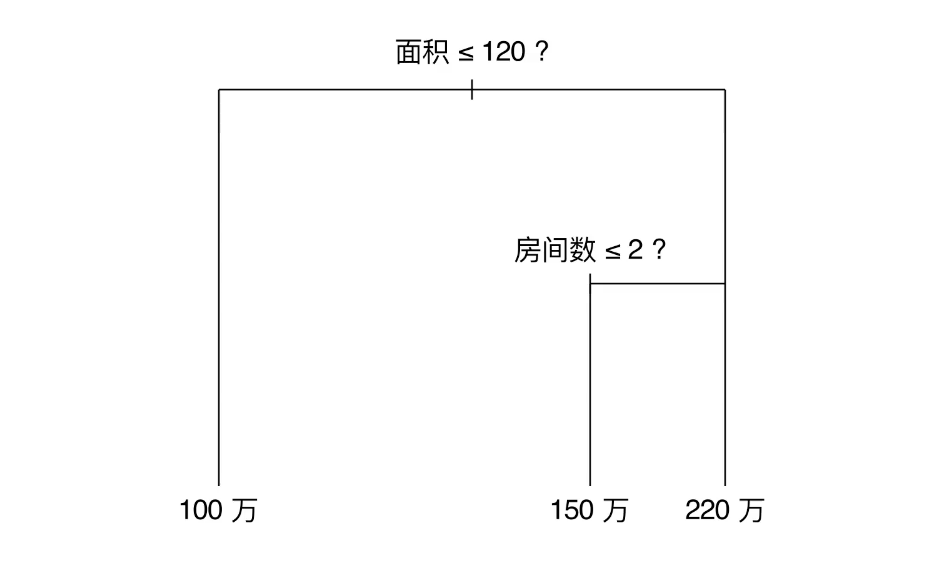
\includegraphics[width=0.5\linewidth,trim=0 0 0 0,clip]{image/regressiontree.png}
  \captionof{figure}{回归树的结构示意图：每个切分对应一个特征阈值，叶子节点给出预测值。}
  \label{fig:regression_tree}
\end{center}
这也就是为什么叫树。

\subsection{回归树的具体计算}
遗憾的是，
要想考虑将特征空间划分为 $J$ 个矩形区域的所有可能性，在计算上是不可行的。
因此一般采用一种 \textbf{自上而下} (top-down) 的 \textbf{贪婪} (greedy) 方法：
\textbf{递归二叉分裂} (recursive binary splitting)。
\begin{definition}[递归二叉分裂]
递归二叉分裂（Recursive Binary Splitting）是一种用于构建回归树和分类树的贪婪算法。其基本思想是：

\begin{enumerate}
  \item 从整个特征空间（即所有训练样本的集合）出发，选择一个特征 $X_j$ 及其切分点 $s$；
  \item 将样本划分为两个矩形区域：
  \[
    R_1(j,s) = \{ x \mid x_j \leq s \}, 
    \qquad
    R_2(j,s) = \{ x \mid x_j > s \} ;
  \]
  \item 选择使得残差平方和（RSS）最小化的分裂：
  \[
    \min_{j,s}\Bigg\{
      \sum_{x_i \in R_1(j,s)} (y_i - \hat{y}_{R_1})^2 \;+\;
      \sum_{x_i \in R_2(j,s)} (y_i - \hat{y}_{R_2})^2
    \Bigg\} ,
  \]
  其中 $\hat{y}_{R_m}$ 表示区域 $R_m$ 内训练样本响应的均值。
  \item 在每个新生成的区域内，重复上述步骤，直到满足停止条件（如区域样本数过小或树的深度达到上限）。
\end{enumerate}

该方法称为“递归”，因为分裂过程会不断重复；称为“二叉”，因为每次分裂都将一个区域划分为两个子区域；称为“贪婪”，因为每次分裂只考虑当前最优，而不是全局最优。
\end{definition}
\begin{dxtips}[贪婪算法-递归二叉分裂]
贪婪算法（Greedy Algorithm）：在每一步选择中，都作出在当前看来最优的局部选择，
而不从整体上进行考虑。
`自上而下'' 指的是从树的顶端（在此处，所有观测值都属于同一个空间）。
开始依次分裂预测变量空间，每个分裂点都会产生两个新的分支。
``贪婪'' 意味着在建立树的每一步中，\textbf{最优} (best) 分裂的确定仅限于这一步进程，
而不是针对全局去选择那些能够在未来过程中构建出更好树的分裂点。
二叉分裂法就是一旦他分割了一次，以后的分割都是在分割好的区域继续分割，不会从两个区域里面个拿出一部分产生一个新的区域即使这样会更好。
\end{dxtips}
\begin{proposition}[防止过拟合想要全局最优]
    上述方法会在训练集中取得良好的预测效果，却很有可能造成数据的过拟合，
导致在测试集上效果不佳。原因在于这种方法产生的树可能过于复杂。
一个分裂点更少、规模更小（区域 $R_1, R_2, \dots, R_J$ 的个数更少）的树
会有更小的方差和更好的可解释性（以增加微小偏差为代价）。

针对上述问题，一种可能的解决办法是：
仅当分裂使残差平方和 RSS 的减小量超过某阈值时，才分裂树节点。
这种策略能生成较小的树，但可能产生短视的问题：
一些起初看起来不值得的分裂在后面可能产生非常好的分裂，
也就是说，在下一步中，RSS 大幅减小。

因此，更好的策略是生成一个很大的树 $T_0$，
然后通过 \textbf{剪枝} (prune) 得到 \textbf{子树} (sub-tree)。
\end{proposition}
\begin{definition}[代价复杂性剪枝]
代价复杂性剪枝（Cost Complexity Pruning，又称最弱链接剪枝 weakest link pruning）
是一种用于从原始大树 $T_0$ 中选择最优子树的策略。该方法不是考虑所有可能的子树，
而是通过引入调整参数 $\alpha \geq 0$，在子树的复杂性和训练误差之间进行权衡。

对于给定的子树 $T$，其代价复杂度定义为：
\[
C_\alpha(T) = \sum_{m=1}^{|T|} \sum_{i: x_i \in R_m} (y_i - \hat{y}_{R_m})^2 \;+\; \alpha |T| ,
\]
其中 $|T|$ 表示子树 $T$ 的终端节点数，$R_m$ 表示第 $m$ 个终端节点对应的区域，
$\hat{y}_{R_m}$ 是区域 $R_m$ 内训练集的平均响应值。

当 $\alpha = 0$ 时，$C_\alpha(T)$ 仅度量训练误差，最优子树为原始大树 $T_0$；
随着 $\alpha$ 增大，终端节点数较多的子树将因复杂性受到惩罚，
使得更小的子树可能成为 $C_\alpha(T)$ 的最优解。
因此，通过调节 $\alpha$ 并最小化 $C_\alpha(T)$，
我们可以在模型复杂度和泛化能力之间找到平衡，从而选出合适的子树。
\end{definition}
也就是最开始的大树太复杂了想砍掉一些枝桠，但是砍的太多就预测的太不准了，砍完枝桠的RSS就是$C_{\alpha}$前面的部分。为了鼓励结构尽可能简单，后面加入T复杂度的权重，权重值为$\alpha$。权重值越高说明越倾向简答的结构。
\begin{dxtips}
    这是一种二次优化的思想，每当想引入新的维度的指标的时候都可以加入带权重的数。这正是 正则化 / 多目标优化 的思想。
\end{dxtips}

\begin{example}[算法 8.1 建立回归树]
\begin{enumerate}
  \item 利用递归二叉分裂在训练集中生成一个大树，只有当终端节点包含的观测值个数低于某个最小值时才停止。
  \item 对大树进行代价复杂性剪枝，得到一系列最优子树，子树是 $\alpha$ 的函数。
  \item 利用 $K$ 折交叉验证选择 $\alpha$。具体做法是将训练集分为 $K$ 折。对所有 $k=1,2,\dots,K$，有：
  \begin{enumerate}
    \item[(a)] 对训练集上所有不属于第 $k$ 折的数据重复步骤 1 和步骤 2，得到与 $\alpha$ 一一对应的子树。
    \item[(b)] 求出上述子树在第 $k$ 折上的均方预测误差。
  \end{enumerate}
  上述操作结束后，每个 $\alpha$ 会有相应的 $K$ 个均方预测误差，对这 $K$ 个值求平均，选出使平均误差最小的 $\alpha$。
  \item 找出选定的 $\alpha$ 值在步骤 2 中对应的子树即可。
\end{enumerate}
\end{example}
\begin{definition}[分类树]
    分类树（classification tree）和回归树十分相似，它们的区别在于：
分类树被用于预测定性变量而非定量变量。也就是研究是什么，而不是是多少的问题。在回归树中，
对一给定观测值，响应预测值取它所属的终端节点内训练集的平均响应值。
与之相对，对分类树来说，给定观测值被预测为它所属区域内的训练集中
最\textbf{常出现的类} (most commonly occurring class)。

\end{definition}
分类树的构造过程和回归树也很像。与回归树一样，分类树采用递归二叉分裂。
但在分类树中，RSS 无法作为确定二叉分裂点的准则。
一个很自然的替代指标是\textbf{分类错误率} (classification error rate)。
既然要将给定区域内的观测值都分到此区域的训练集上最常出现的类中，
那么分类错误率的定义为：此区域的训练集中非最常见类所占的比例。
其表达式如下：
\[
E = 1 - \max_k \big(\hat{p}_{mk}\big),
\tag{8.5}
\]
上式中的 $\hat{p}_{mk}$ 表示第 $m$ 个区域的训练集中的第 $k$ 类所占比例。
但事实上，分类错误率这一指标在构建树时不够敏感。
在实践中，另外两个指标更有优势。
\begin{definition}[基尼系数]
基尼系数（Gini index）用于度量分类树节点的纯度，其定义为
\[
G = \sum_{k=1}^K \hat{p}_{mk} \,(1 - \hat{p}_{mk}),
\tag{8.6}
\]
其中，$\hat{p}_{mk}$ 表示第 $m$ 个区域的训练集中第 $k$ 类所占的比例。

基尼系数可以理解为 $K$ 个类别的总方差。如果所有 $\hat{p}_{mk}$ 的取值都接近于 $0$ 或 $1$，
则基尼系数会很小。因而，基尼系数常被视为度量节点\textbf{纯度} (purity) 的指标：
若基尼系数较小，就意味着该节点包含的观测值几乎都来自同一类。也是Bernoulli 方差 
\end{definition}
\begin{itemize}
  \item $p$ 表示某个类别的占比；
  \item $1-p$ 表示“其他类别的占比”；
  \item $p(1-p)$ 则反映了一个类与其他类的对立程度：
    当分布均衡时（$p$ 和 $1-p$ 接近），该值最大；
    当一边占绝对优势时，该值趋近于 $0$。
\end{itemize}
熵（Entropy）也可以用来替代基尼系数作为分类树分裂指标，其定义为
\[
D = - \sum_{k=1}^K \hat{p}_{mk} \log \hat{p}_{mk},
\tag{8.7}
\]
其中，$\hat{p}_{mk}$ 表示第 $m$ 个区域的训练集中第 $k$ 类所占的比例。

由于 $0 \leq \hat{p}_{mk} \leq 1$，可知 $0 \leq - \hat{p}_{mk}\log \hat{p}_{mk}$。
显然，如果所有 $\hat{p}_{mk}$ 的取值都接近于 $0$ 或 $1$，则熵值接近于 $0$。
因此，与基尼系数类似，如果一个节点的纯度较高，则熵值较小。
事实上，基尼系数和熵在数值上是相当接近的。

在建立分类树的过程中，无论基尼系数还是熵，通常都用于度量某个分裂点的分类质量。
与分类错误率相比，这两种方法对节点纯度更敏感。
上述三种方法都可以用于树的剪枝，但若希望追求较高的预测准确性，最好选择分类错误率。
\section{装代法}
\begin{definition}[装袋法（Bagging）]
在一般情况下难以取得多个训练集，因此可以使用自助法（Bootstrap）作为替代，
即从某一个单一的训练集中重复取样，生成 $B$ 个不同的自助抽样训练集。
然后在第 $b$ 个自助抽样训练集上拟合模型并得到预测值 $\hat{f}^{*b}(x)$。
最后对所有预测值取平均，得到装袋法预测函数：
\[
\hat{f}_{\text{bag}}(x) = \frac{1}{B} \sum_{b=1}^B \hat{f}^{*b}(x).
\]
\end{definition}
决策树（Decision Tree）通常具有较高的方差（high variance），
这意味着如果将同一个训练集随机拆分成两部分，分别建立回归树，
结果可能会差别很大。相比之下，像线性回归这类“简单模型”通常方差较小，
在不同的数据集上结果差别不会太大。为了降低这种高方差，
统计学习里常用一种通用技巧，称为\textbf{自助法聚集}
（bootstrap aggregation），简称\textbf{bagging}。
具体做法是：从训练集里反复有放回地抽样（bootstrap），得到多个子集；
在每个子集上分别建立一个模型（如决策树）；最后把这些模型的预测结果
通过平均或投票的方式组合起来。这样可以显著降低模型的方差，提高泛化性能。
装袋法可以显著改善回归模型的预测效果，尤其对决策树十分有效。
具体做法是：利用 $B$ 个自助抽样训练集分别构造 $B$ 棵回归树，
再对其预测结果取平均。这些树通常根深叶茂且未剪枝，每棵树方差高但偏差小，
通过平均可有效降低方差。事实证明，成百上千棵树的组合能大幅提升预测精度。

在分类问题中，装袋法同样适用。对于一个给定测试样本，记录 $B$ 棵树的预测类别，
再采用\textbf{多数投票}（majority vote），即将出现频率最高的类别作为整体预测结果。
\begin{definition}{袋外误差估计}
装袋法可通过袋外（out-of-bag, OOB）样本直接估计测试误差，而无需交叉验证。
在自助抽样中，每棵树约使用训练样本的三分之二，剩余三分之一即为该树的 OOB 样本。
对某个观测值，可用未包含它的约 $B/3$ 棵树进行预测，并将结果求平均（回归）
或多数投票（分类），得到该观测值的 OOB 预测。综合所有样本即可计算 OOB 均方误差
或分类误差，从而得到装袋法测试误差的有效估计。事实证明，当 $B$ 足够大时，
OOB 误差与留一法交叉验证误差近似等价。
\end{definition}
即使装袋法树的集合比单个树解释数据要困难得多，
也可以用 RSS（针对装袋法回归树）或基尼系数（针对装袋法分类树），
对各预测变量的重要性做出整体概括。
\begin{dxtips}
    bagging和pasting的区别是bagging要把东西放回去，passing不用
\end{dxtips}
\section{随机森林}
\begin{definition}[随机森林]
    随机森林（random forest）通过对树做去相关处理，实现了对装袋法树的改进。
在随机森林中，需要对自助抽样训练集建立一系列决策树，这与装袋法类似。
不过，在建立这些决策树时，每个分裂点不再考虑全部的 $p$ 个预测变量，
而是从中随机抽取 $m$ 个预测变量作为候选。该分裂点所用的预测变量只能从
这 $m$ 个候选变量中选择。在每个分裂点处都要重新抽取 $m$ 个预测变量，
通常 $m \approx \sqrt{p}$。也就是说，每个分裂点所考虑的预测变量个数约等于
总预测变量数的平方根。例如，在 Heart 数据集中共有 $13$ 个预测变量，
则取 $m=4$。
\end{definition}
这个目的就为了防止用装袋法生成的树都长的太相似。比如说都会选择最重要的变量作为顶部分裂点。问题是，与对不相关的量求平均相比，对许多高度相关的量求平均带来的方差减小程度
是无法与前者相提并论的。具体而言，在这种情况下，这意味着装袋法与单个树相比
不会带来方差的明显降低。
但是随机森林因为是随机取出m个预测变量作为候选，那么最强的变量可能都不在里面，这样的话次强变量等等都可能作为顶部分裂点等塑造出不一样的树。
\begin{itemize}
  \item 10 个人都参考同一个答案抄作业 $\;\Rightarrow\;$ 他们错的地方一样，平均结果还是错的。
  \item 10 个人各自独立思考 $\;\Rightarrow\;$ 有人错有人对，平均结果更接近真值。
\end{itemize}
分类聚类然后神经网络把深度学习结合到Matlab上边做边学
\section{boosting提升法}
\begin{definition}[提升法（Boosting）]
提升法（boosting，最初被称为假设提升）是指可以将几个弱学习器组合成一个强学习器的任意集成方法。大多数提升法的总体思想是循环训练预测器，每一次都对其前序预测器做出一些改正。常见的提升法包括 AdaBoost（Adaptive Boosting）和梯度提升（Gradient Boosting）。
\end{definition}
\begin{dxtips}
    Boosting 的核心问题是：如何把多个只比随机猜好一点的弱学习器，
    通过顺序训练和加权组合，提升成一个预测能力强的模型。
\end{dxtips}
\begin{definition}[AdaBoost]
AdaBoost 是一种提升方法，其核心思想是在训练新的预测器时，更多地关注前序预测器欠拟合或分类错误的训练实例。具体而言，算法会先训练一个基础分类器，并用它对训练集进行预测；随后增加被错误分类样本的相对权重，再用更新后的权重训练下一个分类器。如此反复迭代，使后续分类器逐渐专注于前面模型难以处理的样本。
\end{definition}
\begin{align}
\text{初始化样本权重：}\quad 
&w_i^{(1)}=\frac{1}{m},
\qquad
\text{加权错误率：}\quad
r_t=\sum_{i=1}^{m} w_i^{(t)}\mathbf{1}\bigl(h_t(x_i)\neq y_i\bigr)
\\[4pt]
\text{弱分类器权重：}\quad
&\alpha_t=\eta\log\frac{1-r_t}{r_t},
\qquad
\text{样本权重更新：}\quad
w_i^{(t+1)}
=
\frac{
w_i^{(t)}\exp\left(-\alpha_t y_i h_t(x_i)\right)
}{
Z_t
}
\\[4pt]
\text{最终强分类器：}\quad
&H(x)=\operatorname{sign}\left(\sum_{t=1}^{T}\alpha_t h_t(x)\right),
\qquad
\hat{y}(x)
=
\arg\max_{k}
\sum_{\substack{t=1\\ h_t(x)=k}}^{T}
\alpha_t
\end{align}
\begin{dxtips}
    AdaBoost 的核心思想是：提高上一轮被错误分类样本的权重，使后续弱学习器更加关注并修正这些 bad case。提高准确率高的人的话语权。只有第一轮是真正的错误概率后面的都是加权后的错误概率每一轮的优化目标就是加权错误概率最小这个也就是让机器学习的方向。
\end{dxtips}
\begin{note}
在 AdaBoost 中，第 $j$ 个弱学习器的权重可以写为
\[
\alpha_j = \eta \log \frac{1-r_j}{r_j},
\]
其中，$\alpha_j$ 表示第 $j$ 个弱学习器在最终集成模型中的投票权重或可信度；$\eta$ 表示学习率，用来控制每个弱学习器对整体模型的影响程度；$r_j$ 表示第 $j$ 个弱学习器在当前样本权重下的加权错误率；$1-r_j$ 表示其加权正确率；$\frac{1-r_j}{r_j}$ 表示该弱学习器正确分类相对于错误分类的优势比。$r_j$ 越小，说明弱学习器表现越好，此时 $\alpha_j$ 越大，它在最终模型中的话语权也越大。
\end{note}
\begin{dxtips}
    AdaBoost 就像一个军师训练多个谋士。每一轮都会训练一个新谋士，
表现越好的谋士，在最终决策中的投票权越高；
而上一轮被判错的案件，会在下一轮变得更重要，
使新的谋士更倾向于学习如何处理这些 bad case。
\end{dxtips}
\begin{note}
$\eta$ 是人为设定的学习率超参数，用来控制每一轮弱学习器权重的缩放幅度。$\eta$ 越小，模型每轮更新越保守，通常需要更多弱学习器；$\eta$ 越大，模型学习越快，但更容易过拟合。
\end{note}
\begin{dxtips}
    我这样理解对不对Ada boost先用弱分类器训练得到一个模型和他的权重，然后再调整坏的权重然后用另一个弱分类器训练，然后此时两个训练器了。然后最后的决策是他们两商量着做
\end{dxtips}

\begin{definition}[符号函数]
符号函数 $\operatorname{sign}(z)$ 用于判断实数 $z$ 的符号，定义为
\[
\operatorname{sign}(z)
=
\begin{cases}
+1, & z>0,\\
0, & z=0,\\
-1, & z<0.
\end{cases}
\]
在 AdaBoost 中，它用于将多个弱分类器的加权投票结果转化为最终类别。
\end{definition}

\begin{dxtips}
    由于弱分类器优化的加权错误率所以给badcase更高的权重就会尽量保证这个是对的
    
\end{dxtips}
\begin{itemize}
    \item 二分类：使用符号函数判断加权和的正负，$H(x)=\operatorname{sign}\left(\sum_{t=1}^{T}\alpha_t h_t(x)\right)$。
    \item 多分类：统计每个类别的加权投票，选择权重和最大的类别，$\hat{y}(x)=\arg\max_{k}\sum_{\substack{t=1\\ h_t(x)=k}}^{T}\alpha_t$。
\end{itemize}
\subsection{GBRT}
\begin{definition}[梯度提升回归树（Gradient Boosted Regression Tree, GBRT）]
GBRT 是一种基于 Boosting 思想的集成学习算法。它通过迭代训练多棵回归树，使每一棵新树拟合当前模型在损失函数上的负梯度方向，并将这些弱学习器累加形成最终的强预测模型。
\end{definition}

\begin{dxtips}
  \begin{itemize}
    \item 梯度是由函数对各个变量的偏导数组成的向量。
    \item 梯度方向表示函数值上升最快的方向。
    \item 负梯度方向表示函数值下降最快的方向。
\end{itemize}
\end{dxtips}
\begin{dxtips}
    本质就是先把大方向弄正确，每一步都是把新的大方向弄正确，然后慢慢补细节。这个就是第一步先都预测常数使得残差最小，然后由真实值-预测值算出残差，然后用残差训练一个新模型，新模型的指标就是残差最小这个也就是负梯度方向，然后新的函数乘上一个学习率加到前一个函数后面。
\end{dxtips}
\[
\begin{array}{ll}
\text{初始化模型：}
&
F_0(x)=\arg\min_{\gamma}\sum_{i=1}^{m}L(y_i,\gamma)
\\[8pt]

\text{负梯度/伪残差：}
&
r_{im}
=
-\left[
\frac{\partial L(y_i,F(x_i))}
{\partial F(x_i)}
\right]_{F(x)=F_{m-1}(x)}
\\[8pt]

\text{拟合负梯度：}
&
h_m
=
\arg\min_{h}
\sum_{i=1}^{m}
\left(r_{im}-h(x_i)\right)^2
\\[8pt]



\text{模型更新：}
&
F_m(x)
=
F_{m-1}(x)
+
\nu
\sum_{j=1}^{J}
\gamma_{jm}\mathbf{1}(x\in R_{jm})
\end{array}
\]
\begin{dxtips}
  \begin{itemize}
    \item 损失函数 $L(y_i,F(x_i))$：衡量真实值 $y_i$ 与当前模型预测值 $F(x_i)$ 之间的误差，GBRT 每一轮都围绕损失函数下降来更新模型。
    \item 初始模型 $F_0(x)$：GBRT 的初始预测函数，通常是一个常数；在平方误差损失下，它等于所有真实值的平均值。
    \item 负梯度/伪残差 $r_{im}$：第 $m$ 轮中第 $i$ 个样本需要修正的方向；在平方误差损失下，$r_{im}=y_i-F_{m-1}(x_i)$，也就是当前残差。
   
   
    
\end{itemize}
\end{dxtips}
\begin{itemize}
    \item 叶子节点：决策树中样本经过一系列划分后最终落到的终点区域。
    \item $R_{jm}$：第 $m$ 棵树中第 $j$ 个叶子节点对应的样本区域。
    \item $\gamma_{jm}$：第 $m$ 棵树中第 $j$ 个叶子节点的输出值，表示落入该叶子节点的样本统一需要修正的大小。
\end{itemize}
\begin{dxtips}
    每个叶子节点本质上对应一组样本区域，通常需要关注三件事：该叶子包含哪些样本、这些样本当前的残差/负梯度是多少，以及该叶子的输出值 $\gamma$ 是多少。其中真正用于更新模型的是叶子节点的输出值 $\gamma$。如果某个样本落入当前叶子节点管辖的区域，那么该样本在本轮相对于上一版模型的修正量就是 $\nu\gamma$，也就是“学习率 $\nu$ 乘以叶子输出值”。
\end{dxtips}
\begin{dxtips}
    叶子节点可以理解为决策树分叉路径的末端，是模型真正给出输出值的位置。样本从根节点进入树后，会根据每个分裂条件不断向下选择路径，最终落到某个叶子节点；该叶子节点的输出值 $\gamma_{jm}$ 就是这棵树对该样本给出的修正量。
\end{dxtips}
\subsection{XGBoosting}
\dirtree{%
.1 XGBoost 总目标.
.2 目标：让训练损失 + 正则化惩罚最小.
.2 第 $t$ 轮：增加一棵新树 $f_t$.
.3 已固定：前 $t-1$ 棵树.
.4 老树的预测和复杂度都不再优化.
.3 要优化：新树 $f_t$.
.4 新树结构 $q(x)$.
.5 决定样本怎么被分到不同叶子.
.5 通过分裂增益 Gain 判断要不要切分.
.4 叶子输出 $w$.
.5 每个叶子输出一个统一修正值 $w_j$.
.5 固定树结构后，优化每个叶子的 $w_j$.
.5 最优叶子输出：$w_j^*=-\frac{G_j}{H_j+\lambda}$.
.3 更新预测.
.4 新预测 = 旧预测 + 学习率 $\times$ 新树输出.
}
\begin{definition}[XGBoost]
XGBoost（Extreme Gradient Boosting）是一种高效、可扩展的
梯度提升决策树（Gradient Boosting Decision Tree, GBDT）算法实现。
它通过逐轮训练多棵决策树，使每一棵新树修正前面模型的预测误差，
并将所有树的输出累加形成最终预测模型。

相比普通 GBDT，XGBoost 在目标函数中加入了正则化项，
并利用一阶梯度和二阶梯度信息来优化每一轮的树结构与叶子节点权重，
因此通常具有更强的泛化能力、更好的过拟合控制能力和更高的训练效率。
\end{definition}
\begin{dxtips}
    XGBoost他优化的是损失函数是训练损失+正则化，L2正则
\end{dxtips}
\begin{note}[优化函数]
    \[
\mathcal{L}(\phi)
=
\sum_i l(\hat{y}_i,y_i)
+
\sum_k \Omega(f_k)
\]
\end{note}
\begin{dxtips}
训练损失就是：模型在训练样本上预测错了多少。比如回归任务里，常用平方误差。训练目标就是整个目标函数最小
\end{dxtips}
\begin{note}[正则项]
\[
\Omega(f)=\gamma T+\frac{1}{2}\lambda \|w\|^2
\]

\begin{itemize}
    \item $\gamma$：控制叶子节点数量的惩罚强度。$\gamma$ 越大，模型越不愿意继续分裂出新的叶子节点，树会更简单。
    \item $\lambda$：控制叶子节点输出值大小的惩罚强度。$\lambda$ 越大，叶子输出值 $w$ 会被压得越小，模型每一轮更新更加保守。
    \item $T$：这棵树最终有几片叶子，也就是有几个终端节点。
    \item $w$：一棵树所有叶子节点输出值组成的向量。
\end{itemize}

例如一棵树有 3 个叶子节点，输出分别为 $0.8,-0.3,0.1$，则
\[
w=[0.8,\,-0.3,\,0.1],
\qquad
\|w\|^2
=
0.8^2+(-0.3)^2+0.1^2
=
0.74.
\]
\end{note}
\begin{note}[所有树对$ x_i $的输出之和就是预测]
    \[
\hat{y}_i
=
\phi(x_i)
=
\sum_{k=1}^{K} f_k(x_i),
\qquad
f_k \in \mathcal{F}
\]
\end{note}
\begin{note}[加入第t课树的优化函数。]
\[
\mathcal{L}^{(t)}
=
\sum_{i=1}^{n}
l\left(y_i,\hat{y}_i^{(t-1)}+f_t(x_i)\right)
+
\Omega(f_t)
\]

这个其实就是前半部分就是加入 $f_t$ 的以后新的预测与真实的求损失函数，后面的其实就是加入新树的代价，也就是新树的复杂度。因为老树的复杂度已经是固定的了。
\end{note}
\begin{note}
XGBoost 在第 $t$ 轮中，用二阶泰勒展开近似加入新树后的损失函数：
\[
\tilde{\mathcal{L}}^{(t)}
=
\sum_{i=1}^{n}
\left[
g_i f_t(x_i)
+
\frac{1}{2}h_i f_t^2(x_i)
\right]
+
\Omega(f_t)
\]

其中，$g_i$ 是一阶梯度，表示当前预测应该往哪个方向修正；$h_i$ 是二阶梯度，表示损失函数在当前位置的曲率信息；$f_t(x_i)$ 是新树对第 $i$ 个样本给出的修正量。

这一步的作用是把原本不好直接优化的损失函数，近似成关于 $f_t(x_i)$ 的二次形式，从而方便后面求叶子节点最优权重和分裂增益。
\end{note}
\begin{example}[梯度如何影响计算]
以平方误差 $l(y_i,\hat{y}_i)=(\hat{y}_i-y_i)^2$ 为例，对 $\hat{y}_i$ 求导得到一阶梯度 $g_i=2(\hat{y}_i-y_i)$。若 $y_i=10,\hat{y}_i=6$，则 $g_i=2(6-10)=-8$，负梯度 $-g_i=8$，说明预测值应该往上调。

但新树不是给每个样本单独记修正量，而是把相似样本分到同一个叶子，并输出统一修正值。例如样本 1 的负梯度是 $8$，样本 3 的负梯度是 $2$，若它们落入同一叶子，则叶子可能输出折中值 $5$。当学习率 $\eta=0.1$ 时，实际更新为 $0.1\times 5=0.5$，所以样本 1 和样本 3 都加 $0.5$。因此，梯度只告诉模型修正方向和需求强弱，最终改多少由叶子输出、学习率和正则化共同决定。
\end{example}
\begin{dxtips}
    本质上就是把ft（xi）当成了Δx，然后损失函数是固定的比如这个例子里面就是平方误差。他的二阶导就是2
\end{dxtips}
\begin{note}
    二次函数求最小值：对 $w_j$ 求导，令导数等于 $0$：
\[
G_j + (H_j+\lambda)w_j = 0,
\qquad
w_j^*
=
-
\frac{G_j}{H_j+\lambda}.
\]

这就是叶子节点最优输出值。
\end{note}
\begin{note}[分裂增益 Gain]
XGBoost 用分裂增益判断一个节点是否值得继续切分：
\[
Gain
=
\frac{1}{2}
\left[
\frac{G_L^2}{H_L+\lambda}
+
\frac{G_R^2}{H_R+\lambda}
-
\frac{G^2}{H+\lambda}
\right]
-
\gamma
\]

其中，$G_L,H_L$ 是左子节点的一阶、二阶梯度之和，$G_R,H_R$ 是右子节点的一阶、二阶梯度之和，$G,H$ 是父节点的一阶、二阶梯度之和。$\lambda$ 控制叶子权重的 L2 正则，$\gamma$ 是新增叶子的复杂度惩罚。

如果 $Gain>0$，说明这一刀能让目标函数下降，值得切分；如果 $Gain\le 0$，说明这一刀不划算，不切。
\end{note}
\subsection{LightGBM}
\dirtree{%
.1 LightGBM 总目标.
.2 目标：在保持 GBDT 精度的同时，让训练更快、内存更省.
.2 本质：仍然是 GBDT / GBM.
.3 每一轮增加一棵新树.
.3 新树仍然拟合当前模型的负梯度 / 残差.
.3 仍然通过分裂增益判断节点怎么切分.
.2 核心瓶颈：普通 GBDT 找分裂太慢.
.3 对每个特征都要扫描大量样本.
.3 复杂度大致受 $\#data \times \#feature$ 影响.
.3 数据越大、特征越多，训练越慢.
.2 加速一：Histogram 直方图算法.
.3 连续特征先离散成 bin.
.4 不再枚举所有连续取值.
.4 只在有限个 bin 上找切分点.
.3 构建直方图复杂度：$O(\#data \times \#feature)$.
.3 找切分点复杂度：$O(\#bin \times \#feature)$.
.2 加速二：GOSS，减少样本数量.
.3 按梯度绝对值排序样本.
.4 大梯度样本：模型还没学好，信息量大.
.4 小梯度样本：模型已经学得比较好，信息量小.
.3 保留前 $a \times 100\%$ 的大梯度样本.
.3 从剩余小梯度样本中随机采样 $b \times 100\%$.
.3 对采到的小梯度样本乘上权重 $\frac{1-a}{b}$.
.4 目的：补偿被丢掉的小梯度样本.
.4 尽量不改变原始数据分布.
.3 用近似增益 $\tilde{V}_j(d)$ 代替全量增益 $V_j(d)$.
.2 加速三：EFB，减少特征数量.
.3 利用稀疏特征的互斥性.
.4 很多 one-hot 特征不会同时非零.
.4 可以把互斥特征打包成一个 bundle.
.3 特征数从 $\#feature$ 变成 $\#bundle$.
.3 复杂度从 $O(\#data \times \#feature)$ 降到 $O(\#data \times \#bundle)$.
.2 最终效果.
.3 GOSS 处理样本多的问题.
.3 EFB 处理特征多的问题.
.3 Histogram 让分裂搜索更快.
.3 所以 LightGBM = 更轻、更快的 GBDT 实现.
}
\begin{dxtips}
     \(V_j(d)\) 是全量样本上的真实分裂增益；\(\tilde{V}_j(d)\) 是 GOSS 采样后的近似分裂增益。   
\end{dxtips}
\begin{definition}[原始分裂增益 $V_j(d)$]
$V_j(d)$ 表示在第 $j$ 个特征上，以 $d$ 为切分点时的分裂增益：
\[
V_j(d)
=
\frac{1}{n}
\left[
\frac{
\left(\sum_{x_i:x_{ij}\le d} g_i\right)^2
}{
n_l^j(d)
}
+
\frac{
\left(\sum_{x_i:x_{ij}>d} g_i\right)^2
}{
n_r^j(d)
}
\right].
\]
它用全量样本计算该切分点的收益，是 GOSS 近似分裂增益 $\tilde{V}_j(d)$ 要近似的对象。
\end{definition}
\begin{definition}[核心公式：GOSS 近似分裂增益Gradient-based One-Side Sampling]
GOSS发生在抉择要不要分叉的时候。
在 GOSS 中，先保留梯度绝对值最大的 前百分a的样本，记为集合 $A$；
再从剩余的小梯度样本中随机采样 百分之b，记为集合 $B$。
然后用下面的近似分裂增益代替全量数据上的分裂增益：
\[
\tilde{V}_j(d)
=
\frac{1}{n}
\left[
\frac{
\left(
\sum_{x_i\in A_l} g_i
+
\frac{1-a}{b}
\sum_{x_i\in B_l} g_i
\right)^2
}{
n_l^j(d)
}
+
\frac{
\left(
\sum_{x_i\in A_r} g_i
+
\frac{1-a}{b}
\sum_{x_i\in B_r} g_i
\right)^2
}{
n_r^j(d)
}
\right].
\]
其中：
Al就是left梯度前百分之a的点，Ar就是右边前百分之a点，第 \(j\) 个特征在切分点 \(d\) 上的分裂增益。比如在年龄这个特征 25分裂的收益，$n$ 是当前这个节点里的样本总数，
左边的样本数就是 $n_l^j(d)$ 个，
右边的样本数就是 $n_r^j(d)$ 个。

这里 $g_i$ 表示第 $i$ 个样本的梯度；
$a$ 表示保留的大梯度样本比例；
$b$ 表示从小梯度样本中采样的比例；
$\frac{1-a}{b}$ 是小梯度样本的放大系数，用来补偿没有被采到的小梯度样本。
\end{definition}
\begin{dxtips}
    因为是和的平方，个数从原来的n变成了n²所以最外面还得再除一次n
\end{dxtips}
\begin{dxtips}
   \begin{itemize}
    \item GOSS 变快，是因为它不用让所有小梯度样本都参与分裂增益计算。
    
    \item 大梯度样本：模型还没学好，信息量大，所以全部保留。
    
    \item 小梯度样本：模型已经学得比较好，信息量小，所以只抽一部分。
    
    \item 被抽中的小梯度样本：乘上一个放大系数，代表那些没被抽中的小梯度样本。
\end{itemize}
\end{dxtips}
\begin{note}
    这个长的像顺序统计量，前百分之a本来就是顺序统计量的表述。这个vj就是从原来每一个都要取每一个权重都一样变成了取一部分。
\end{note}
\begin{example}
    

$d$ 表示某个特征上的切分点。

例如，如果特征是年龄，切分点是 $25$，那么：
\[
\text{年龄} \le 25 \quad \text{走左边},
\qquad
\text{年龄} > 25 \quad \text{走右边}.
\]
\end{example}


\begin{dxtips}[$\frac{1-a}{b}$ 的无偏补偿]
GOSS 只采样一部分小梯度样本，所以直接求和会低估小梯度样本的总体贡献。
乘上 $\frac{1-a}{b}$ 后，有
\[
\mathbb{E}\left[
\frac{1-a}{b}
\sum_{x_i\in B} g_i
\right]
=
\sum_{x_i\in A^c} g_i.
\]
因此，$\frac{1-a}{b}$ 的作用是让采样小梯度的加权和成为全体小梯度梯度和的无偏估计。

\end{dxtips}
\begin{definition}[Histogram 直方图算法]
Histogram 直方图算法是 LightGBM 用来加速分裂搜索的方法。
它先将连续特征离散成有限个 bin，
然后在训练决策树时不再枚举所有连续取值作为切分点，
而只在 bin 的边界上寻找最佳切分点。

因此，构建直方图的复杂度为
\[
O(\#data \times \#feature),
\]
寻找切分点的复杂度为
\[
O(\#bin \times \#feature).
\]
由于通常有 $\#bin \ll \#data$，
所以 Histogram 可以显著加快分裂点搜索。
\end{definition}

\begin{definition}[EFB：互斥特征捆绑]
EFB（Exclusive Feature Bundling）利用高维稀疏特征的互斥性，
把多个几乎不会同时非零的特征合并成更少的 bundle。

设原始特征数为 $\#feature$，捆绑后的特征组数为 $\#bundle$，
且通常有
\[
\#bundle \ll \#feature.
\]
因此，直方图构建复杂度可以从
\[
O(\#data \times \#feature)
\]
降低为
\[
O(\#data \times \#bundle).
\]
\end{definition}
\begin{dxtips}
    \begin{itemize}
    \item Histogram：把每个连续特征的取值离散成若干个 bin。
    目的：减少每个特征上的候选切分点数量，也就是减少 $d$ 的数量。
    
    \item EFB：把多个互斥的稀疏特征打包成一个 bundle。
    目的：减少有效特征数量，也就是减少 $j$ 的数量。
\end{itemize}

\[
\begin{array}{ll}
\text{原来要搜索：} & \text{所有特征 } j \times \text{所有切分点 } d \\[4pt]
\text{Histogram 后：} & \text{所有特征 } j \times \text{少量 bin 切分点 } d \\[4pt]
\text{EFB 后：} & \text{少量 bundle } j \times \text{少量 bin 切分点 } d
\end{array}
\]
\end{dxtips}








\begin{example}[EFB 合并互斥 one-hot 特征]
假设广告/推荐场景中有城市 one-hot 特征：
\[
\text{北京},\ \text{上海},\ \text{深圳},\ \text{广州}.
\]
同一用户同一时刻只属于一个城市，因此这些特征互斥。例如
\[
\text{北京}=1 \Rightarrow \text{上海}=\text{深圳}=\text{广州}=0.
\]

原始特征为：
\[
\begin{array}{c|cccc}
\text{用户} & \text{北京} & \text{上海} & \text{深圳} & \text{广州} \\
\hline
A & 1 & 0 & 0 & 0 \\
B & 0 & 1 & 0 & 0 \\
C & 0 & 0 & 1 & 0 \\
D & 0 & 0 & 0 & 1
\end{array}
\]
EFB 可将其捆绑成一个特征 $\text{城市\_bundle}$：
\[
\text{北京}\mapsto 1,\quad
\text{上海}\mapsto 2,\quad
\text{深圳}\mapsto 3,\quad
\text{广州}\mapsto 4.
\]
捆绑后：
\[
\begin{array}{c|c}
\text{用户} & \text{城市\_bundle} \\
\hline
A & 1 \\
B & 2 \\
C & 3 \\
D & 4
\end{array}
\]

因此，特征数从 $4$ 降为 $1$，直方图构建复杂度从
\[
O(\#data \times 4)
\quad \text{降为} \quad
O(\#data \times 1).
\]
\end{example}
\begin{dxtips}[不是一类合并成一类而是只要互斥就可以放在一类]
EFB 可以理解为训练前的“合并同类项”：
它把许多很少同时出现的稀疏特征列，打包成更少的 bundle 特征。

但 EFB 的合并依据不是语义类别，例如并不是因为
\[
\text{北京},\text{上海},\text{深圳},\text{广州}
\]
都属于城市，所以才合并。

它真正关心的是特征之间是否互斥，即：
\[
x_a \neq 0 \quad \Rightarrow \quad x_b \approx 0.
\]

如果两个特征几乎不会同时非零，就可以放入同一个 bundle。bundle也就是特征束也就是在训练前先简化分化，分类以后改变映射关系从而矩阵的维度
\end{dxtips}
\begin{note}
    于是，直方图不只是统计每个桶里的样本数，
还会把同一个桶中的梯度累加起来：
\[
\begin{array}{c|c|c}
\text{桶} & \text{样本数} & \sum g_i \\
\hline
\text{桶1} & 1 & -2 \\
\text{桶2} & 2 & 1+3=4 \\
\text{桶3} & 1 & -1 \\
\text{桶4} & 1 & 2
\end{array}
\]

这张按桶汇总样本数和梯度信息的统计表，
就是 LightGBM 中所说的直方图。
\end{note}
\begin{theorem}[LightGBM 的 Leaf-wise 生长策略]
LightGBM 采用 leaf-wise 的树生长策略。
在每一步分裂时，它不会像 level-wise 那样按层同时扩展所有叶子节点，
而是优先选择当前分裂增益最大的叶子节点继续分裂。

因此，leaf-wise 通常可以更快降低训练损失，
但也更容易生成较深的局部路径，从而带来过拟合风险。
实际训练中通常需要通过
\[
\texttt{num\_leaves},\quad \texttt{max\_depth}
\]
等参数控制树的复杂度。
\end{theorem}
\begin{note}[LightGBM 常用复杂度控制参数]
Leaf-wise 生长会优先分裂增益最大的叶子节点，
因此训练损失下降快，但也更容易长出过深的局部路径。
实际训练中通常用以下参数控制模型复杂度：
\begin{itemize}
    \item $\texttt{num\_leaves}$：控制一棵树最多有多少个叶子节点，是 leaf-wise 中最重要的复杂度参数。
    \item $\texttt{max\_depth}$：限制树的最大深度，防止某些路径过深。
    \item $\texttt{min\_data\_in\_leaf}$：限制每个叶子节点至少包含多少样本，防止叶子过小导致过拟合。
    \item $\texttt{learning\_rate}$：控制每棵新树对模型的修正幅度，越小越保守，通常需要更多树。
    \item $\texttt{lambda\_l1},\ \texttt{lambda\_l2}$：分别表示 L1 和 L2 正则化，用来惩罚模型复杂度。
\end{itemize}
\end{note}
\begin{dxtips}
EFB 的关键不只是“把互斥特征打包”，还包括两个细节：
\textbf{冲突率（conflict rate）} 和 \textbf{图着色（graph coloring）}。

实际数据中，并不是所有特征都能做到完全互斥。
LightGBM 允许少量特征冲突，只要冲突率足够低，
这些特征仍然可以被放进同一个 bundle。

为了找到合适的 bundle，LightGBM 会把特征看成图中的节点。
如果两个特征不能互斥，就在它们之间连边。
这样，寻找最少 bundle 的问题就可以转化为图着色问题：
相互冲突的特征不能使用同一种颜色，同一种颜色对应一个 bundle。
实际算法中通常使用贪婪策略近似求解。
\end{dxtips}
\chapter{训练神经网络}
\chapter{调优与上线意识}